\begin{center}
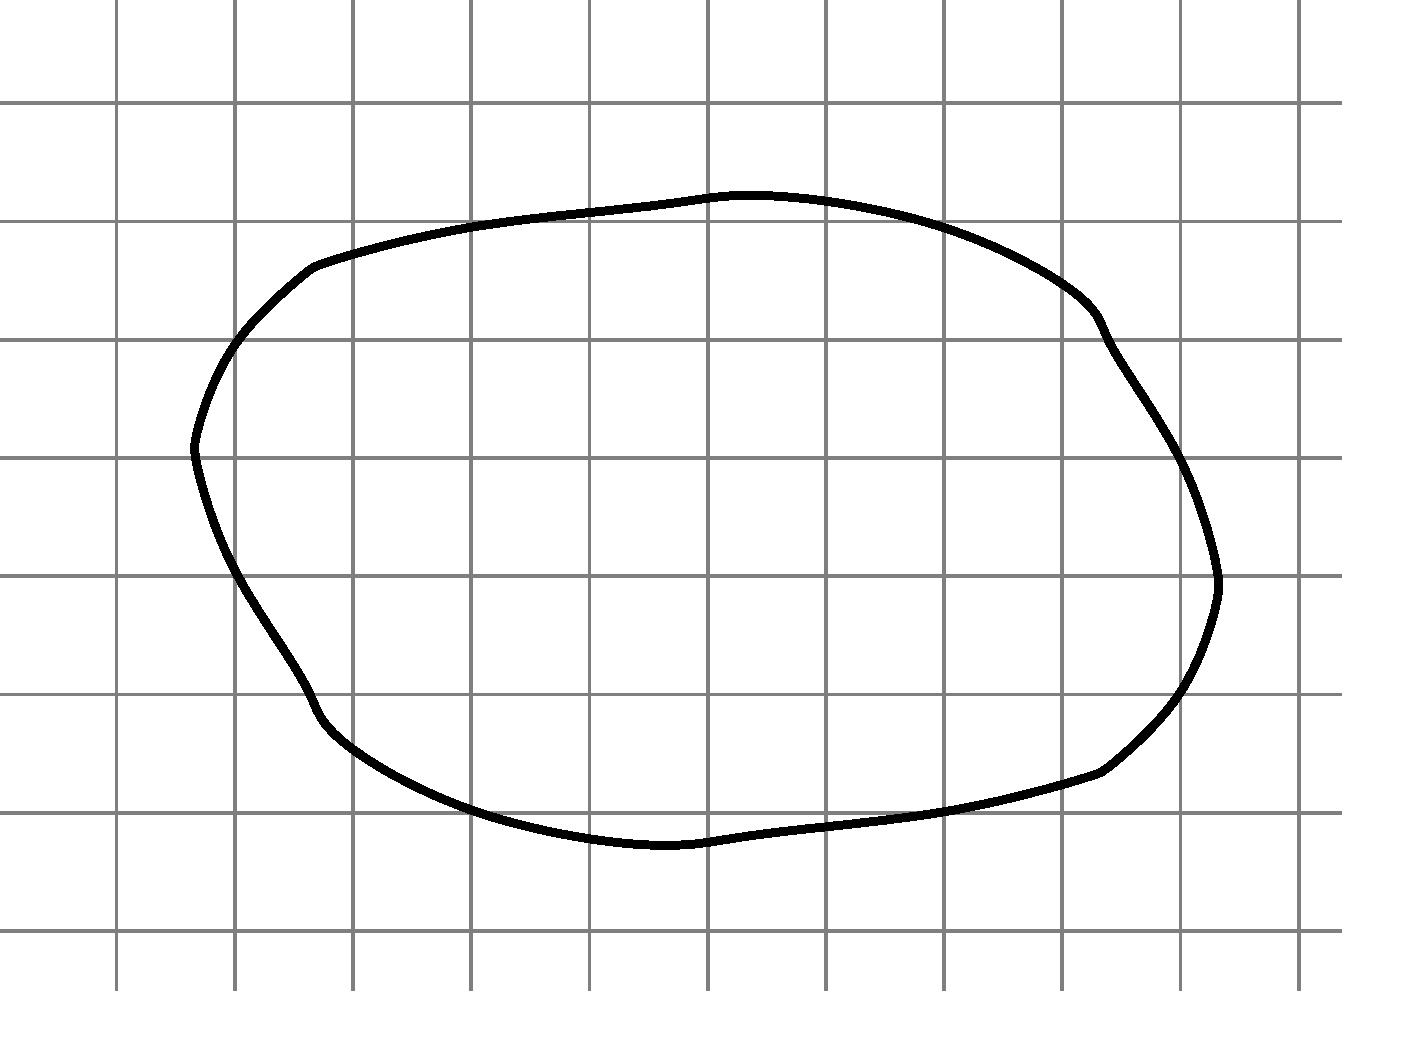
\includegraphics[width=0.6\textwidth]{./Figures/tiled_room.pdf}
\end{center}

Suppose you have an oddly shaped room with square tiles, and you want to estimate its square footage. Let $n$ be the number of full tiles you count, and let $m$ stand for the number of broken tiles. Denote the area of a single tile -- which can be computed: it is the square of the side length -- by $A_0$. Then we have the lower and upper bounds
\[n \cdot A_0 \leq A \leq (n+m) \cdot A_0\]
for the area $A$ of the room. Now, convince yourself that this estimate would be better (tighter), if the tiles were smaller\footnote{Mark the areas $n \cdot A_0$ and $(n+m) \cdot A_0$ in the sketch above, and then think about what would happen if we had tiles of half the side length}!

Finding areas under curves or volumes under surfaces is called \emph{integration}. It is one of the most fundamental and important concepts of mathematics, and it has applications in every scientific discipline. The above approach of approximating areas with large numbers of simple pieces can be quite cumbersome. Fortunately, there is very powerful connection to differentiation, which allows to compute integrals in a more efficient way.

\begin{application}[Centre of mass]
A large metal plate of uniform thickness and the shape in the sketch (let us call it $S$; the area under $f(x)=\sqrt{x}$ for $x$ from $0$ to $9$) needs to be balanced on a single point.
\begin{center}
	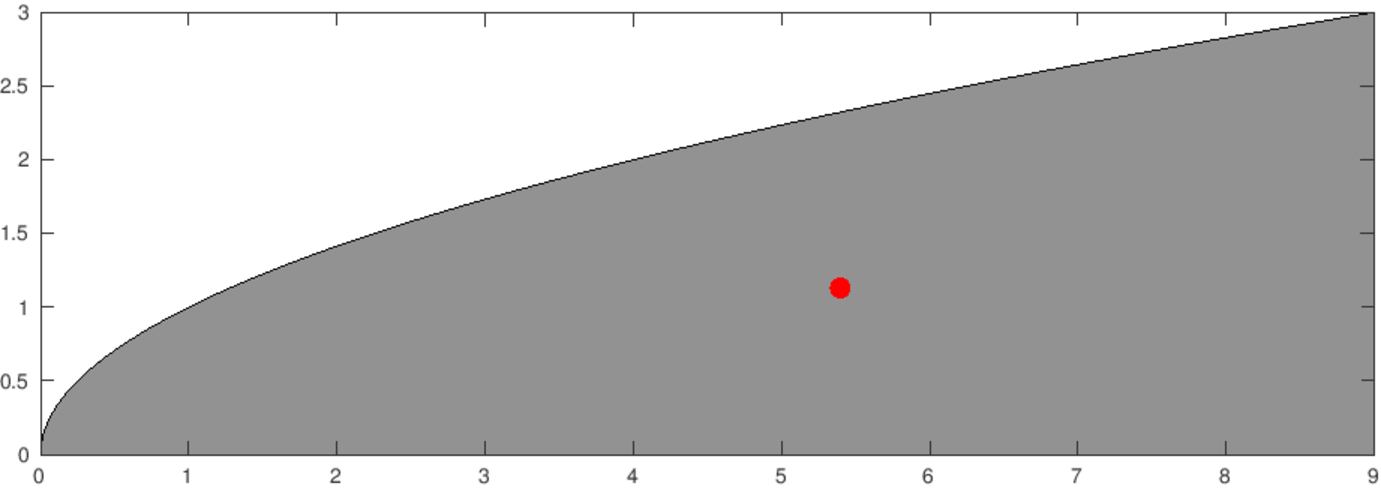
\includegraphics[width=0.6\textwidth]{./Figures/centre_of_mass.pdf}
\end{center}
That is, the centre of mass of $S$ needs to be found.

This can be solved with integration: The $x$ and $y$ coordinates of the centre of mass of $S$ are
\begin{align*}
x_c &= \frac{\iint_S x \: \d A}{\iint_S 1 \: \d A} = 5.4, \\
y_c &= \frac{\iint_S y \: \d A}{\iint_S 1 \: \d A} = 1.125.
\end{align*}
We will learn how to compute those integrals in this chapter.
\end{application}


\section{Theory of Integration in One Dimension}

\begin{definition}[Definite Integral, Riemann Sum]
Let $f(x)$ be continuous on $a \le x \le b$ and divide the interval
$[a,b]$ into $n$ subintervals of equal width $\Delta x = \rfrac{(b-a)}{n}$. Let
\[ x_0 = a, \:\: x_1 = a + \Delta x, \:\: x_2 = x_1 + \Delta x = x_0 + 2 \Delta x, \:\:
\dots, \:\: x_n = x_0 + n \Delta x = b \]
be the endpoints of these subintervals. 
\begin{enumerate}[(i)]
\item
Then the \emph{definite integral} of $f$ from $a$ to $b$ is defined as
\begin{equation}
\label{eq:def_itgr}
\itgr{a}{b}{f(x)}{x} := \lim_{n \to \infty} \sum_{j=1}^{n} f(c_j) \Delta x,
\end{equation}
where $x_{j-1} \le c_j \le x_{j}$. Here $f(x)$ is called the \emph{integrand}, $a$ the lower boundary, and $b$ the upper boundary.
\item
The sum appearing in the above definition is called a \emph{Riemann sum} of $f$ over $[a,b]$. If the points $c_j$ are always chosen to be the right-hand end point of their subinterval, that is $c_j=x_j$, we obtain the right-hand Riemann sum
\[ \sum_{j=1}^{n} f(x_j) \Delta x. \]
Using the left end points of the subintervals, $c_j=x_{j-1}$, gives the left-hand Riemann sum
\[ \sum_{j=1}^{n} f(x_{j-1}) \Delta x = \sum_{j=0}^{n-1} f(x_{j}) \Delta x. \]
\end{enumerate}	
\end{definition}

\begin{remark}
\label{rem:def_int}
\begin{enumerate}[(i)]
	\item Equation~\eqref{eq:def_itgr} introduces a new quantity -- the definite integral of $f$ over $[a,b]$ -- and \emph{defines} (that is what the ``$:=$'' means) it to be equal to the limit for $n \rightarrow \infty$ of the Riemann sums on the right. Note that on the right-hand side of \eqref{eq:def_itgr}, different choices could be made for the points $c_j$. One should therefore show now that all these possible different choices lead to the same limit. That is, one should show that $\itgr{a}{b}{f(x)}{x}$ as defined above is \emph{well-defined}! This will be given as an exercise at the end of this section.
	\item The following figure illustrates the right-hand Riemann sum for $n=4$, 
	\[ \sum_{j=1}^{4} f(x_j) \Delta x, \]
	of some function $f$.
	\figbox{Right-hand Riemann sum of $f$ for $n=4$:}
	The rectangles in this figure have areas ``height'' $\cdot$ ``width'' 
	$= f(x_j)\cdot \Delta x$, and they are added up to obtain the Riemann sum. For comparison, the left-hand Riemann sum is
	\figbox{Left-hand Riemann sum of $f$ for $n=4$:}
	We see that in both cases, the Riemann sums approximate the area under the curve $y=f(x)$, and as in the example of the oddly-shaped room in the introduction, those approximations will get better if we choose $n$ to be larger. We can therefore interpret their limit, i.e., $\itgr{a}{b}{f(x)}{x}$, as the signed area under the curve $y=f(x)$:
	\figbox{Definite integral of $f$ over the integral $[a,b]$:}
	Here, the word ``signed'' was added since areas below the $x$-axis contribute negatively to the definite integral.
\end{enumerate}
\end{remark}

\begin{example}
Consider $f(x)=	\rfrac35 \, x$, $a=0$, $b=5$. First, let us find the left-hand Riemann sum for $n=5$ of $f$. The partition of $[a,b]=[0,5]$ is
\begin{equation*}
\begin{split}
\Delta x &= \frac{b-a}{n} = \frac{5-0}{5} = 1,\\
x_0 &= 0, \: x_1 = 1, \: x_2 = 2, \: \dots, x_5 = 5,
\end{split}
\end{equation*}
and therefore
\begin{equation*}
\begin{split}
\itgr{0}{5}{\frac{3}{5} \, x}{x} & \approx \sum_{j=0}^4 f(x_j) \Delta x 
= [f(0)+f(1)+f(2)+f(3)+f(4)] \cdot 1 \\
& = \frac35 \, [0+1+2+3+4] = 6.
\end{split}
\end{equation*}
We now generalise this computation to find the definite integral $f$ over the interval $[a,b]$.
The partition of the interval is
\begin{equation*}
\begin{split}
\Delta x &= \frac{b-a}{n} = \frac{5-0}{n} = \frac{5}{n},\\
x_0 &= 0, \: x_1 = \frac{5}{n}, \: x_2 = 2\frac{5}{n}, \: \dots, x_n = n\frac{5}{n}=5,
\end{split}
\end{equation*}
and therefore
\begin{equation*}
\begin{split}
\itgr{0}{5}{\frac{3}{5} \, x}{x} & = \lim_{n \to \infty} \sum_{j=0}^{n-1} f(x_j) \Delta x 
= \lim_{n \to \infty} \frac{5}{n} \sum_{j=0}^{n-1} \frac{3}{5} x_j  \\
& = \lim_{n \to \infty} \frac{5}{n} \sum_{j=0}^{n-1} \frac{3}{5} \frac{5}{n} \, j
= \lim_{n \to \infty} \frac{15}{n^2} \sum_{j=0}^{n-1} j \\
& = \lim_{n \to \infty} \frac{15}{n^2} \frac{(n-1)n}{2}
= \lim_{n \to \infty} \frac{15}{2} \frac{n-1}{n} = 7.5,
\end{split}
\end{equation*}
Note that this result agrees with the area
\[ A = \frac{3\cdot5}{2}, \]
found by noticing that the region under the curve $y=f(x)$ is a right-angled triangle.
\end{example}

\begin{properties}
\label{prop:di}
Let $a,b,\alpha\in\mathbb{R}$, $a<b$, and let $f(x),g(x)$ be continuous functions on $[a,b]$. Then:
\begin{equation*}
\begin{split}
(1) \qquad & \itgr{a}{a}{f(x)}{x} = 0, \\
(2) \qquad & \itgr{a}{b}{f(x)}{x} = -\itgr{b}{a}{f(x)}{x}, \\
(3) \qquad & \itgr{a}{b}{[f(x)+g(x)]}{x} = \itgr{a}{b}{f(x)}{x} + \itgr{a}{b}{g(x)}{x}, \\
(4) \qquad & \itgr{a}{b}{\alpha \cdot f(x)}{x} = \alpha \cdot \itgr{a}{b}{f(x)}{x}, \\
(5) \qquad & \itgr{a}{b}{f(x)}{x} = \itgr{a}{c}{f(x)}{x} + \itgr{c}{b}{f(x)}{x}  \\
(6) \qquad & \text{If~} f(x) \ge 0 \text{~on~} [a,b] \text{,~then} \itgr{a}{b}{f(x)}{x} \ge 0.
\end{split}
\end{equation*}
Now suppose that $f(x)$ is continuous on the interval $[-a,a]$, where $a>0$. Then we have
\begin{equation*}
\begin{split}
(7) \qquad & \text{If $f(x)$ is even, i.e. $f(-x)=f(x)$, then} 
	\itgr{-a}{a}{f(x)}{x} = 2\itgr{0}{a}{f(x)}{x}, \\
(8) \qquad & \text{If $f(x)$ is odd, i.e. $f(-x)=-f(x)$, then} \itgr{-a}{a}{f(x)}{x} = 0.
\end{split}
\end{equation*}
\end{properties}

\begin{remark}
\begin{enumerate}[(i)]
	\item All those properties are proven starting from the definition~\ref{eq:def_itgr} of the definite integral. (There is nothing else to start from, is there?) Only the proof of the last property is written out below.
	\item Properties (3) and (4) state that integration is \emph{linear}, and they can by proven by using the corresponding laws for sums and limits (e.g., pull the constant $\alpha$ out of the sum and then out of the limit in definition~\ref{eq:def_itgr}).
\end{enumerate}	
\end{remark}

\begin{proof}
For the proof of (8), we consider an odd function and we use only even $n$ for the limit $n\to\infty$. Since all choices for the points $c_j$ lead to the same limit, we make a choice that suits our purpose well: let the $c_j$ be the midpoints of their subintervals. The Riemann sums are
\[ \sum_{j=1}^n f(c_j) \Delta x 
= \Delta x \cdot \left[ f(c_1) + f(c_2) + \dots f(c_{n-1}) + f(c_n) \right], \]
and comparing to 
\figbox{An odd function and its Riemann sum, using midpoints:}
we see that this Riemann sum is zero since $f(c_1)+f(c_n)=0$, $f(c_2)+f(c_{n-1})=0$, \ldots This gives 
\[ \itgr{-a}{a}{f(x)}{x} = \lim_{n \to \infty} 0 = 0.\]

Now, the above assertion that $f(c_{j})+f(c_{n-j+1})=0$ seems to be confirmed by the sketch, but we should prove it properly: After working out formulas for the partition points $x_j$, we find
\[ c_j = -a+\Delta x\left(j-\frac12\right) = -a+\frac{2a}{n}\left(j-\frac12\right) \]
for the midpoints $c_j$ of the subintervals. This gives
\begin{equation*}
\begin{split}
c_{n-j+1} & = -a+\frac{2a}{n}\left(n-j+1-\frac12\right) \\
& = -a+2a+\frac{2a}{n}\left(-j+\frac12\right) = -c_j,
\end{split}
\end{equation*}
and therefore, since $f$ is odd,
\[ f(c_j)+f(c_{n-j+1})=f(c_j)+f(-c_j)=f(c_j)-f(c_j) = 0. \]
\end{proof}

\begin{definition}[Mean]
For continuous $f:[a,b]\rightarrow\mathbb{R}$, the real number
\[ \bar{f}:= \frac{1}{b-a} \itgr{a}{b}{f(x)}{x} \]
is called the \emph{mean} or \emph{average} of $f$ over the interval $[a,b]$.
\end{definition}

\begin{remark}
We have
\[ \bar{f}\cdot(b-a) = \itgr{a}{b}{f(x)}{x}, \]
that is, the area under the constant function $\bar{f}$ over $[a,b]$ is the same as the area under the graph of $f$:
\figbox{Definite integrals of $f$ and of the constant function $\bar{f}$:}
Note that this is similar for the average of numbers -- if Alice has an average of $\bar{m}$ on all the tests in a module, and Bob scored exactly $\bar{m}$ each time, then they have the same total mark.
\end{remark}

\begin{theorem}[Mean Value Theorem (MVT)]
Let $f:[a,b]\rightarrow\mathbb{R}$ be continuous. Then there exists a point $c\in(a,b)$ such that
\[ f(c) = \frac{1}{b-a} \itgr{a}{b}{f(x)}{x}. \]
That is, $f$ attains its mean value at some point in $(a,b)$.
\end{theorem}

\begin{proof}
Let
\[ M:=\max_{x\in[a,b]} f(x), \qquad m:=\min_{x\in[a,b]} f(x).\]
Since $f$ is continuous, it takes every value between $m$ and $M$. Therefore, we need to show that
\begin{equation}
\label{eq:proof_mvt}
 m \le \bar{f} \le M.
\end{equation}
We have
\begin{equation*}
\begin{split}
& M-f(x) \ge 0 \qquad \text{on~} [a,b] \\
\stackrel{\text{prop. (6)}}{\Longrightarrow} \quad & \itgr{a}{b}{M-f(x)}{x} \ge 0 \\
\stackrel{\text{prop. (3)}}{\Longrightarrow} \quad & \itgr{a}{b}{M}{x}-\itgr{a}{b}{f(x)}{x} \ge 0 \\
\Longrightarrow \quad & \itgr{a}{b}{f(x)}{x} \le \itgr{a}{b}{M}{x} = M(b-a).
\end{split}
\end{equation*}
Combining this with the outcome of the analogous computation for $f(x)-m$ gives
\[ m(b-a) \le \itgr{a}{b}{f(x)}{x} \le M(b-a). \]
Division by $(b-a)$ gives the inequality~\ref{eq:proof_mvt}, and hence completes the proof.
\end{proof}

\begin{definition}[Area Function]
For continuous $f:[a,b]\rightarrow\mathbb{R}$, the \emph{area function}
\[ A : [a,b] \rightarrow \mathbb{R} \]
of $f$ is
\[ A(x):=\itgr{a}{x}{f(t)}{t}. \]
\end{definition}

\begin{remark}
We use the variable $t$ in the integrand to avoid confusion with the variable of $A$.
\figbox{The area function for a continuous function $f$:}
\end{remark}

\begin{theorem}[Fundamental Theorem of Calculus (FTC)]
Let $f:[a,b]\rightarrow\mathbb{R}$ be continuous.
\begin{enumerate}[(i)]
	\item The derivative of the area function is
	\[ A'(x) = \Df{}{x} A(x) = f(x).\]
	That is,
	\[ \Df{}{x} \itgr{a}{x}{f(t)}{t} = f(x). \]
	\item If $F$ is any \emph{antiderivative} of $f$, i.e. a function with $F'(x)=f(x)$, then
	\[ \itgr{a}{b}{f(x)}{x} = F(b) - F(a). \]
\end{enumerate}
\end{theorem}

\begin{example}
We solve the following definite integral by guessing a function whose derivative is the integrand. Once this guessed antiderivative is written down, one should always check whether it really differentiates to the original integrand. 
\begin{equation*}
\begin{split}
\itgr{1}{3}{(x^3-6x)}{x} 
& = \left( \eval{\frac{x^4}{4} - 3x^2}{1}{3} \right) 
	\qquad \left[ \text{check :~} \Df{}{x} \left( \frac{x^4}{4} - 3x^2 \right) 
	= x^3-6x \quad \text{\checkmark} \right] \\
& = \left( \frac{3^4}{4} - 3\cdot 3^2 \right)
- \left( \frac{1^4}{4} - 3\cdot 1^2 \right) 
= \frac{81}{4} - 27 - \frac{1}{4} + 3 = -4
\end{split}
\end{equation*}
The vertical line in the second expression stands for ``evaluate at $x=3$ and then subtract the evaluation at $x=1$'' -- as on the right-hand side of FTC (ii). To foreshadow the proof of the FTC, note that the choice of antiderivative is not unique, but different choices seem to be leading to the same result; e.g.,
\[ \itgr{1}{3}{x^3-6x}{x} = \left( \eval{\frac{x^4}{4} - 3x^2 + 42}{1}{3} \right)
= \frac{81}{4} - 27 + 42 - \frac{1}{4} + 3 - 42 = -4. \]
\end{example}

\begin{proof}
\begin{enumerate}[(i)]
	\item Using the definition of the derivative, the definition of the area function, and property (5) of the definite integral, we obtain
	\[ A'(x) = \lim_{h \to 0} \frac{A(x+h)-A(x)}{h}
	= \lim_{h \to 0} \frac{1}{h} \itgr{x}{x+h}{f(t)}{t}. \]
	The expression within the limit on the right is the average of $f$ over the interval $[x,x+h]$. By the MVT, there exist $c_h\in[x,x+h]$ such that
	\[ f(c_h) = \frac{1}{h} \itgr{x}{x+h}{f(t)}{t}. \]
	This allows to continue the computation of $A'(x)$ above as follows:
	\begin{equation*}
	\begin{split}
	A'(x) & = \lim_{h \to 0} f(c_h) \qquad \text{where~} c_h\in[x,x+h] \\
		  & = f\left(\lim_{h \to 0} c_h \right) = f(x). \\	
	\end{split}
	\end{equation*}
	\item The area function $A(x)$ is an antiderivative of $f$ -- by (i) -- and for it, the claim is true by definition:
	\[ A(b) - A(a) = A(b) = \itgr{a}{b}{f(t)}{t}. \]
	Now let $F(t)$ be a different antiderivative of $f$. Then
	\[ \Df{}{x} \left( F(x) -A(x) \right) = f(x) -f(x) = 0, \]
	and therefore $F$ and $A$ differ only by a constant,
	\[ F(x) = A(x) + c.\]
	This gives
	\[ F(b) - F(a) = (A(b)+c) - (A(a)+c) = A(b)-A(a) = \itgr{a}{b}{f(t)}{t}. \]
\end{enumerate}
\end{proof}

\begin{corollary}
\label{thm:cor_ftc}
\begin{enumerate}[(i)]
	\item \[ \itgr{a}{b}{F'(t)}{t} = F(b)-F(a). \]
	\item \[ \Df{}{x} \itgr{a(x)}{b(x)}{f(t)}{t} = f(b(x))\,b'(x) - f(a(x))\,a'(x). \]
\end{enumerate}
\end{corollary}

\begin{remark}
\begin{enumerate}[(i)]
	\item The word ``corollary'' is usually used for results that follow from important theorems.
	\item The first identity is also called the ``Total Change Theorem'', and it follows immediately from FTC (ii). It reads: ``Integrating the rate of change of a function over an interval gives the total change over that interval.'' 
	\item Make sure to take note of the second identity -- it is important for differentiating more complicated integral expressions. It follows from the chain rule:
	\begin{equation*}
	\begin{split}
	\Df{}{x} \itgr{c}{b(x)}{f(t)}{t} & = \Df{}{x} \itgr{c}{y}{f(t)}{t} \qquad\qquad (y=b(x)) \\
	& = \Df{}{y} \itgr{c}{y}{f(t)}{t} \cdot \Df{y}{x} \qquad\qquad (\text{chain rule})\\
	& = f(y) \cdot \Df{y}{x} = f(b(x))\,b'(x),
	\end{split}
	\end{equation*}
	and using property (5) of the definite integral, we can prove the formula in full generality, that is, for the case when the lower bound is a function of $x$ as well.
\end{enumerate}	
\end{remark}

\begin{definition}[Indefinite Integral]
The \emph{indefinite integral}
\[ \itgr{}{}{f(x)}{x} \]
of $f(x)$ is the collection of all antiderivatives of the function $f$.
\end{definition}

\begin{example}
\begin{enumerate}[(i)]
	\item For 
	\[ F(x) = \itgr{1}{x^3}{t^5}{t}, \]
	we find, identifying $f(t)=t^5$ and using the formula from theorem~\ref{thm:cor_ftc},
	\[ F'(x) = \Df{}{x} \itgr{1}{x^3}{f(t)}{t}
	= f(x^3)\cdot\Df{}{x}\left(x^3\right) - f(1)\cdot\Df{}{x}(1) 
	= \left(x^3\right)^5 \cdot 3x^2 + 0 = 3x^{17}. \]
	
	We can check this by finding $F(x)$ explicitly,
	\[ F(x) = \itgr{1}{x^3}{t^5}{t} 
	= \left(\left. \frac{t^6}{6} \right|_1^{x^3}\right)
	= \frac{\left(x^3\right)^6}{6} - \frac{1}{6}, \]
	and then differentiating:
	\[ F'(x) = \Df{}{x} \left( \frac{x^{18}}{6} - \frac{1}{6} \right) 
	= 18\cdot\frac{x^{17}}{6} - 0 = 3x^{17} \quad \text{\checkmark}\]
	\item \[ \itgr{}{}{\e^{3x}}{x} = \frac{1}{3} \e^{3x} + c. \]
	Here, we use the constant $c$ as a place holder to cover all the infinitely many possible antiderivatives, e.g.
	\[ \frac{1}{3} \e^{3x}, \quad \frac{1}{3} \e^{3x} - 5, \quad
	\frac{1}{3} \e^{3x} + 117.38, \quad \dots, \]
	of $f(x)=\e^{3x}$.
\end{enumerate}	
\end{example}

\begin{remark}
We conclude this section with the following remarks:
\begin{enumerate}[(i)]
	\item Integration is ``the opposite of differentiation''.
	\item Integrals with boundaries are definite integrals, and then the result is a real number.
	\item Integrals without boundaries are indefinite integrals, and then the result is a function! Make sure to not forget the constant of integration!
\end{enumerate}
\end{remark}

\begin{exercise}
\begin{enumerate}[(i)]
	\item Interpret the properties~\ref{prop:di} -- perhaps add a few sketches to your notes -- and prove one or two of them.
	\item Find the area function $A_0$ of $f(x)=x^3-6x$ with $a=0$. Then set $a=1$ and find the corresponding area function $A_1$. Compare $A_0$ and $A_1$ to each other and to the indefinite integral of\footnote{A$A_0(x)$ and $A_1(x)$ should differ by the constant $\rfrac{-11}{4}$ -- where does this number come from? By choosing the constant of integration suitably, you should be able to obtain both $A_0$ and $A_1$ from the indefinite integral.} $f(x)$.
	\item Find the definite integral
	\[ \itgr{0}{1}{\e^x}{x} \]
	using Riemann sums\footnote{You will need the formula for the sum of the first $n$ terms of the geometric series.}, and then compare to the value found via direct integration.
	\item Show that the definite integral, \eqref{eq:def_itgr}, is well-defined\footnote{Cf. remark~\ref{rem:def_int} for the meaning of `well-defined'' in this context. For fixed $n$, we obtain the largest possible Riemann sum by letting the $c_j$ be the points at which $f$ takes its maximal value on $[x_{j-1},x_j]$. Similarly for the smallest possible Riemann sum. What is the difference between those two extremes, and what happens for $n\to\infty$?}.
	\item Find the derivative of\footnote{Careful, the FTC can not immediately by applied, because the $x$ appears in the integrand as well. Hence pull out the $x$ and then differentiate the product $x \cdot \int_0^{x^2}\dots$. Note that there is a different way to solve this: find an explicit formula for $F$ in terms of $x$ -- without an integral -- and then differentiate. Try this approach as well and make sure your answers agree!}
	\[ F(x) = \itgr{0}{x^2}{x}{t}. \]
\end{enumerate}
\end{exercise}


\section{Methods of Integration}

\subsection{Basic Integrals}

\begin{properties}[Basic Integrals]
\label{prop:bi}
\begin{equation*}
\begin{split}
(1) \qquad & \itgr{}{}{x^r}{x} = \frac{x^{r+1}}{r+1} + c \qquad \text{for~} r\not=-1,  \\
(2) \qquad & \itgr{}{}{\frac{1}{x}}{x} = \ln\abs{x} + c, \\
(3) \qquad & \itgr{}{}{\e^x}{x} = \e^x + c, \\
(4) \qquad & \itgr{}{}{a^x}{x} = \frac{a^x}{\ln a} + c \qquad \text{for~} a>0,  \\
(5) \qquad & \itgr{}{}{\cos x}{x} = \sin x + c, \\
(6) \qquad & \itgr{}{}{\sin x}{x} = -\cos x + c, \\
(7) \qquad & \itgr{}{}{\frac{1}{\cos^2 x}}{x} = \tan x + c, \\
(8) \qquad & \itgr{}{}{\frac{1}{\sin^2 x}}{x} = -\cot x + c, \\
(9) \qquad & \itgr{}{}{\frac{1}{1+x^2}}{x} = \arctan x + c, \\
(10) \qquad & \itgr{}{}{\frac{1}{\sqrt{1-x^2}}}{x} = \arcsin x + c, \\
(11) \qquad & \itgr{}{}{\cosh x}{x} = \sinh x + c, \\
(12) \qquad & \itgr{}{}{\sinh x}{x} = \cosh x + c. 
\end{split}
\end{equation*}
\end{properties}

\begin{remark}
\begin{enumerate}[(i)]
	\item The function $\arctan x$ is the inverse function of $\tan x$. It is sometimes denoted $\tan^{-1}$, but this carries potential for confusion, as $\arctan x \not= \rfrac{1}{\tan x}$ ! Similarly, for $\cos x$ and $\sin x$ and their inverse functions. The expressions appearing in (7) and (8) could be rewritten using the conventions
	\[  \sec x = \frac{1}{\cos x}, \quad \csc x = \frac{1}{\sin x}, \quad
	\cot x = \frac{\cos x}{\sin x}.\]
	\item The linearity properties (3) and (4) of \ref{prop:di} remain true for indefinite integrals. Therefore, we can now integrate all linear combinations of functions appearing in the integrands of properties~\ref{prop:bi}.
	\item All the integrals above are verified by differentiating the antiderivative on the right and comparing to the integrand on the left. For example,
	\[ \Df{}{x} (-\cos x + c) = \sin x, \]
	and hence (6) is correct.
	\item Formula (2) can be used to evaluate definite integrals such as $\itgr{1}{2}{\rfrac{1}{x}}{x}$ or $\itgr{-23}{-5}{\rfrac{1}{x}}{x}$, but definite integrals across $x=0$ are not permitted since $f(x) = \rfrac1x$ is not defined at $x=0$. This means that in this context, $x$ is either always positive or always negative. This allows to verify (2) by considering two cases: \\
	{\it Case (a):} $x>0$ \\
	\phantom{abc}If $x$ is positive, then $\abs{x}=x$ and
	\[ \Df{}{x} (\ln \abs{x} + c) = \Df{}{x} \ln x = \frac1x \qquad \text{\checkmark} \]
	{\it Case (b):} $x<0$ \\
	\phantom{abc}If $x$ is negative, then $\abs{x}=-x$ and we obtain
	\[ \Df{}{x} (\ln \abs{x} + c) = \Df{}{x} \ln(-x) = \frac{1}{-x}\cdot(-1) = \frac1x \]
	\phantom{abc}as well.
\end{enumerate}
\end{remark}

\begin{example}
\begin{enumerate}[(i)]
	\item
	\begin{equation*}
	\begin{split}
	\itgr{}{}{ x^{11} + 5\cos x - 7^x }{x} 
	& = \itgr{}{}{x^{11}}{x} + 5\itgr{}{}{\cos x}{x} - \itgr{}{}{7^x}{x} \\
	& = \frac{x^{12}}{12} + 5\sin x - \frac{7^x}{\ln 7} + c.
	\end{split} 
	\end{equation*}
	\item \[ \itgr{1}{\e}{\frac1x}{x} = \eval{ \ln \abs{x} }{1}{\e} = \ln e - \ln 1 = 1, \]
	which some calculus text books use to define the constant $\e\approx2.718$.
\end{enumerate}
\end{example}

\begin{remark}
In the following example, recognising an expression coming from the chain rule allows us to ``guess'' an integral:
\[ \itgr{}{}{2x\,\cosh(x^2)}{x} = \sinh(x^2)+c. \]
The next theorem makes the application of this idea more systematic.
\end{remark}

\subsection{Substitution}

\begin{theorem}[Substitution] 
\label{thm:subst}
If $u=u(x)$ is differentiable and $f$ continuous, then
\begin{enumerate}[(i)]
	\item \[ \itgr{}{}{f(u(x)) \cdot u'(x) }{x} = \itgr{}{}{f(u)}{u}. \]
	\item \[ \itgr{a}{b}{f(u(x)) \cdot u'(x) }{x} = \itgr{u(a)}{u(b)}{f(u)}{u}. \]
\end{enumerate}
\end{theorem}

\begin{example}
\begin{enumerate}[(i)]
	\item \begin{equation*}
	\begin{split}
	\itgr{}{}{x\,\left(1+x^2\right)^{13}}{x} & 
		\qquad \qquad \qquad \qquad \left[ \begin{array}{rcl}
		u & = & 1+x^2 \\ 1 \cdot \d u & = & 2x \cdot \d x \\
		\rightarrow \: x \d x & = & \rfrac12 \, \d u
		\end{array}\right] \\
	& = \itgr{}{}{u^{13}\,\frac12}{u} \\ 
	& = \frac12 \frac{u^{14}}{14} + c 
	  = \frac{\left( 1 + x^2 \right)^{14}}{28} + c. 
	\end{split}
	\end{equation*}
	Check:
	\[ \Df{}{x} \left( \frac{\left( 1 + x^2 \right)^{14}}{28} + c \right)
	= \frac{14}{28} \left( 1 + x^2 \right)^{14-1} \cdot 2x
	= x\,\left( 1 + x^2 \right)^{13} \qquad \text{\checkmark}\]
	\item \begin{equation*}
	\begin{split}
	\itgr{0}{\rfrac{\pi}{2}}{\cos(\cos x)\sin x}{x} &  
		\qquad \qquad \qquad \left[ \begin{array}{rcl}
		u & = & \cos x \\ \d u & = & -\sin x \, \d x \\
		\rightarrow \: \sin x \, \d x & = & - \d u \\
		u=0 & \leftrightarrow & x = \rfrac\pi2\\
		u=1 & \leftrightarrow & x = 0\\
		\end{array}\right] \\
	& = \itgr{1}{0}{\cos u \cdot (-1)}{u} \\ 
	& = \itgr{0}{1}{\cos u}{u} = \eval{\sin u}{0}{1}   
	  = \sin 1. 
	\end{split}
	\end{equation*}
	\item \begin{equation*}
	\begin{split}
	I = \itgr{0}{\sqrt{3}}{\e^{\sqrt{1+x^2}}\frac{x}{\sqrt{1+x^2}}}{x} &  
		\qquad \qquad \qquad \left[ \begin{array}{rcl}
		u & = & \sqrt{1+x^2} \\ \d u & = & \frac{x}{\sqrt{1+x^2}} \d x \\
		u=2 & \leftrightarrow & x = \sqrt{3}\\
		u=1 & \leftrightarrow & x = 0\\
		\end{array}\right] \\
	& = \itgr{1}{2}{\e^u}{u} \\ 
	& = \eval{\e^u}{1}{2} = \e^2-\e^1 = \e(\e-1).
	\end{split}
	\end{equation*} 
	Alternatively, one could leave the boundaries in terms of $x$ and evaluate the antiderivative after substituting back to $x$:
	\[ I = \eval{\e^u}{\cdot}{\cdot} = \eval{\e^{\sqrt{1+x^2}}}{0}{\sqrt{3}}
	= \e^{\sqrt{1+3}} - \e^{\sqrt{1}} = \e(\e-1). \]
\end{enumerate}	
\end{example}

\begin{remark}
In the integrands of the previous examples, we have seen the inner functions
\[ 1+x^2, \quad \cos x, \quad \sqrt{1+x^2}, \]
to which the outer functions
\[ x^{13}, \quad \cos x, \quad \e^x, \]
respectively, are applied. A first attempt for solving integrals of that kind should always be to substitute for the identified inner function. The question is then whether the other factors in the integrand are absorbed by the transformation of the differential $\d\cdot$. If not, then more work or a different approach is required.
\end{remark}

\begin{example}
\label{expl:arctan-int}
Compute the indefinite integral
\[ I = \itgr{}{}{\frac{1}{4+x^2}}{x}. \]
Note that we could read off the answer immediately from the list in properties~\ref{prop:bi} if the $4$ in the denominator was a $1$. We therefore bring the integral in that form using substitution:
\begin{equation*}
\begin{split}
I = \itgr{}{}{\frac{1}{4+x^2}}{x}
& = \itgr{}{}{\frac{1}{4\left(1+\rfrac{x^2}{4}\right)}}{x} \\
& = \frac{1}{4} \itgr{}{}{\frac{1}{1+\left(\rfrac{x}{2}\right)^2}}{x}
\qquad \qquad \qquad \left[ \begin{array}{rcl}
u & = & \rfrac{x}{2} \\ \d u & = & \rfrac{1}{2} \, \d x \\
\end{array}\right] \\
& = \frac{1}{2} \itgr{}{}{\frac{1}{1+u^2}}{u} \\ 
& = \frac{1}{2} \arctan u + c = \frac{1}{2} \arctan \left(\frac{x}{2} \right) + c.
\end{split}
\end{equation*} 
\end{example}

\subsection{Trigonometric Identities}

\begin{properties}[Trigonometric Identities]
\label{prop:ti}
\begin{equation*}
\begin{split}
(1) \qquad & \cos^2 x + \sin^2 x = 1,  \\
(2) \qquad & \cos(x+y) = \cos x \cos y - \sin x \sin y, \\
(3) \qquad & \sin(x+y) = \sin x \cos y + \cos x \sin y, \\
(4) \qquad & \cos(2x) = 2\cos^2 x - 1 = 1 - 2 \sin^2 x, \\
(5) \qquad & \sin(2x) = 2\sin x \cos x, \\
(6) \qquad & 2\sin x \cos y = \sin(x-y)+\sin(x+y), \\
(7) \qquad & 2\cos x \cos y = \cos(x-y)+\cos(x+y), \\
(8) \qquad & 2\sin x \sin y = \cos(x-y)-\cos(x+y), \\
(9) \qquad & \cosh^2 x - \sinh^2 x = 1, \\
\end{split}
\end{equation*}
\end{properties}

\begin{example}
\begin{enumerate}[(i)]
	\item \begin{equation*}
	\begin{split}
	\itgr{0}{\pi}{\sin^2 x}{x} & = \itgr{0}{\pi}{\sin x \cdot \sin x}{x} 
	\stackrel{(8)}{=} \itgr{0}{\pi}{\frac12 \left[\cos(x-x)-\cos(x+x)\right]}{x} \\
	& = \itgr{0}{\pi}{\frac12 \left[\cos(0)-\cos(2x)\right]}{x}
	= \frac12 \itgr{0}{\pi}{ 1-\cos(2x)}{x} \\
	& = \frac12 \left( \eval{x-\rfrac12 \sin(2x)}{0}{\pi} \right) = \frac{\pi}{2}.
	\end{split}
	\end{equation*}
	A better way to compute this integral would be to use the identity (4) -- this allows to go directly from the first expression to the fifth.
	\item \begin{equation*}
	\begin{split}
	\itgr{}{}{\cos^4 x}{x} & = \itgr{}{}{\left( \cos^2 x \right)^2}{x} 
	\stackrel{(4)}{=} \itgr{}{}{\left( \frac{\cos(2x)+1}{2} \right)^2}{x} \\
	& = \itgr{}{}{\frac14 \left(\cos^2(2x)+2\cos(2x)+1\right)}{x} \\
	& \stackrel{(4)}{=} \itgr{}{}{\frac14 \left(\frac{\cos(4x)+1}{2}+2\cos(2x)+1\right)}{x} \\
	& = \frac{1}{32} \sin(4x) + \frac14 \sin(2x) + \frac38 x + c.
	\end{split}
	\end{equation*}
	\item 
	\[ \itgr{}{}{\sin(2x)\sin(7x)}{x} 
	\stackrel{(8)}{=} \itgr{}{}{\frac12 \left[ \cos(-5x) - \cos(9x) \right]}{x}
	= \frac{\sin(5x)}{10} - \frac{\sin(9x)}{18} + c. \]
	\item The following example contains a typical substitution with trigonometric functions, and some comments on it will be made in the next remark. \begin{equation*}
	\begin{split}
	\itgr{2.5}{5}{\frac{\sqrt{25-x^2}}{x^2}}{x} &  
		\qquad \qquad \qquad \qquad \qquad \qquad \left[ \begin{array}{rcl}
		x & = & 5\sin\theta \\ \d x & = & 5\cos\theta \, \d \theta \\
		x=5 & \leftrightarrow & \theta = \rfrac{\pi}{2} \\
		x=2.5 & \leftrightarrow & \theta = \rfrac{\pi}{6}\\
		\end{array}\right] \\
	& = \itgr{\rfrac{\pi}{6}}{\rfrac{\pi}{2}}
	{\frac{\sqrt{25-(5\sin\theta)^2}}{(5\sin\theta)^2}\,5\cos\theta}{\theta} \\ 
	& = \itgr{\rfrac{\pi}{6}}{\rfrac{\pi}{2}}
	{\frac{\sqrt{1-\sin^2\theta}}{\sin^2\theta}\,\cos\theta}{\theta} 
	\stackrel{(1)}{=} \itgr{\rfrac{\pi}{6}} {\rfrac{\pi}{2}}{\frac{\cos^2\theta}{\sin^2\theta}}{\theta} \\
	& \stackrel{(1)}{=} \itgr{\rfrac{\pi}{6}}{\rfrac{\pi}{2}}
	{\frac{1-\sin^2\theta}{\sin^2\theta}}{\theta} 
	= \itgr{\rfrac{\pi}{6}}{\rfrac{\pi}{2}}{\frac{1}{\sin^2\theta}-1}{\theta} \\
	& = \eval{-\cot \theta - \theta}{\rfrac{\pi}{6}}{\rfrac{\pi}{2}}
	= - 0 - \frac{\pi}{2} + \frac{\rfrac{\sqrt{3}}{2}}{\rfrac{1}{2}} + \frac{\pi}{6} 
	= \sqrt{3} - \frac{\pi}{3}.
	\end{split}
	\end{equation*}
	\item \begin{equation*}
	\begin{split}
	\itgr{}{}{\frac{1}{\sqrt{x^2-a^2}}}{x} &  
		\qquad \qquad \qquad \qquad \qquad \qquad \left[ \begin{array}{rcl}
		x & = & a\cosh t \\ \d x & = & a\sinh t \, \d t \\
		\end{array}\right] \\
	& = \itgr{}{}{\frac{a\sinh t}{\sqrt{(a\cosh t)^2-a^2}}}{t} \\
	& \stackrel{(9)}{=} \itgr{}{}{1}{t} = t+c = \text{arccosh} \left( \frac{x}{a} \right) + c.
	\end{split}
	\end{equation*}
\end{enumerate}
\end{example}

\begin{remark}
\begin{enumerate}[(i)]
	\item Note the similarities in the approaches for (iv) and (v) above, and also note the differences: In both cases, we have square roots of expressions $\pm(a^2-x^2)$ in the integrand, and we use the trigonometric Pythagoras formula (1) of properties~\ref{prop:ti} and the corresponding hyperbolic version $(9)$ to simplify them. The following thoughts might help you to avoid confusion of the two. For $\sqrt{a^2-x^2}$, we need $x$ to be small, namely in the range $[0,a]$, and the trigonometric functions have a bounded range. For $\sqrt{x^2-a^2}$, we need $x$ to be large, and the function $g(t) = a\cosh t$ has the correct range, $ R(g) = [a,\infty)$.
	\item For our next integration method, we apply the product rule to differentiate the product $fg$, and then bring one of the terms on the other side,
	\[ f'g = (fg)' - fg'.\]
	Integrating this expression with respect to $x$, we obtain the following result.
\end{enumerate}
\end{remark}

\subsection{Integration by Parts}

\begin{theorem}[Integration by Parts]
\[ \itgr{}{}{f'(x)g(x)}{x} = f(x)g(x) - \itgr{}{}{f(x)g'(x)}{x}. \]
\end{theorem}

\begin{example}
\begin{enumerate}[(i)]
	\item 
	The integration by parts formula allows us to find an import integral that was missing in properties~\ref{prop:bi} -- the integral of the logarithm:
	\begin{equation*}
	\begin{split}
	\itgr{}{}{\ln x}{x} 
	& =	\itgr{}{}{\underbrace{1}_{\text{int.}} \cdot \underbrace{\ln x}_{\text{diff.}}}{x}
	= x\ln x - \itgr{}{}{x \cdot \Df{}{x}(\ln x)}{x} \\
	& = x\ln x - \itgr{}{}{x\cdot\frac{1}{x}}{x}
	= x\ln x - \itgr{}{}{1}{x} = x\ln x - x + c.
	\end{split}
	\end{equation*}
	We have integrated $\ln x$ by differentiating it!
	\item \begin{equation*}
	\begin{split}
	\itgr{}{}{\underbrace{x^2}_{\text{diff.}} \underbrace{\e^{3x}}_{\text{int.}}}{x} 
	& = \frac13\e^{3x}x^2 - \itgr{}{}{\frac13\e^{3x}2x }{x}
	= \frac13\e^{3x}x^2 - \frac23 \left[ 
	\itgr{}{}{\underbrace{\e^{3x}}_{\text{int.}}\underbrace{x}_{\text{diff.}} }{x} \right] \\
	& = \frac13\e^{3x}x^2 - \frac23 
	\left[ \frac13 \e^{3x}x - \itgr{}{}{\frac13\e^{3x}}{x}  \right] \\
	& = \frac13\e^{3x}x^2 - \frac23 
		\left[ \frac13 \e^{3x}x - \frac19\e^{3x} + \wtd{c} \right] 
	= \frac13 \e^{3x} \left[ x^2-\frac23x+\frac29 \right] + c.
	\end{split}
	\end{equation*}
	\item When applying integration by parts to definite integrals, all terms need to be evaluated over the interval; e.g.,
	\begin{equation*}
	\begin{split}
	\itgr{0}{1}{\underbrace{x}_{\text{diff.}}\underbrace{(1+x)^{17}}_{\text{int.}}}{x} 
	& = \eval{x\frac{(1+x)^{18}}{18}}{0}{1} - \itgr{0}{1}{\frac{(1+x)^{18}}{18}}{x} \\
	& = 1 \cdot \frac{2^{18}}{18}-0-\frac{1}{18 \cdot 19} 
		\left( \eval{(1+x)^{19}}{0}{1} \right) \\
	& = \frac{1}{18 \cdot 19} \left( 19 \cdot 2^{18} - 2^{19} + 1 \right)
	= \frac{495161}{38}.
	\end{split}
	\end{equation*}
	\item \begin{equation*}
	\begin{split}
	I & = \itgr{}{}{\underbrace{\e^x}_{\text{int.}}\underbrace{\cos x}_{\text{diff.}}}{x} 
	= \e^x\cos x - \itgr{}{}{\e^x (-\sin x)}{x} \\
	& = \e^x\cos x + \itgr{}{}
		{\underbrace{\e^x}_{\text{int.}}\underbrace{\sin x}_{\text{diff.}}}{x} \\
	& = \e^x\cos x + \e^x\sin x - \itgr{}{}{\e^x \cos x}{x} \\
	& = \e^x\cos x + \e^x\sin x - I
	\end{split}
	\end{equation*}
	This computation does not seem to lead anywhere, as the integral we need to compute reappears after two applications of the integration by parts rule. Differentiating $\e^x$ and integrating the trigonometric term instead, leads to a similar situation. However, we can solve the equation for $I$ ! This gives
	\[ I = \itgr{}{}{\e^x \cos x}{x} = \frac12 \e^x(\cos x + \sin x) +c.\]
\end{enumerate}
\end{example}

\begin{remark}
\begin{enumerate}[(i)]
	\item When faced with an integrand that contains a power of $x$ and other, more complicated terms, one should first try substitution. If this does not work, integration by parts is the next best option. In this case, one would usually choose the power of $x$ as the term that is to be differentiated -- the reason for this is that differentiation makes powers simpler and repeated integration by parts will eventually dispose of them. However, there are no firm rules for integration and one should remain open-minded to non-standard approaches.
	\item Many of the examples above are specifically designed so that the computations work out relatively smoothly. In general, integration is quite hard and sometimes even impossible. It is therefore important to keep in mind that differentiation provides a straight-forward way to verify the integrals you have found. Here is an integral that cannot be solved:
	\[ \itgr{}{}{\e^{-x^2}}{x}. \]
	\item Consider the computation
	\[ \frac{2}{x+4}-\frac{3}{x-1} 
	= \frac{2(x-1)-3(x+4)}{(x+4)(x-1)} = \frac{-(x+14)}{x^2+3x-4}, \]
	and note that, while we can integrate the expression on the left-hand side -- e.g.,
	\[ \itgr{}{}{\frac{2}{x+4}}{x} = 2\ln(x+4) + c \]
	-- the expression on the right is not covered by the integration methods we have developed so far. Reversing finding the common denominator therefore extends the set of functions we can integrate. This is called integration by partial fractions.
\end{enumerate}
\end{remark}

\subsection{Partial Fractions}

\begin{example}
\label{expl:partial_fractions}
\begin{enumerate}[(i)]
	\item Find the integral
	\[ I = \itgr{}{}{\frac{2x+16}{x^2+2x-35}}{x}. \]
	{\it Sol.:}
	\begin{equation*}
	\begin{split}
	\frac{2x+16}{x^2+2x-35} & =\frac{2x+16}{(x-5)(x+7)}
	= \frac{A}{x-5} +\frac{B}{x+7} \\
	& = \frac{A(x+7)+B(x-5)}{(x-5)(x+7)}
	= \frac{(A+B)x+(7A-5B)}{(x-5)(x+7)}
	\end{split}
	\end{equation*}
	\[ \Longrightarrow \quad \begin{cases} A+B &= 2 \\ 7A-5B &= 16 \end{cases} 
		\qquad \Longrightarrow \quad 
		\begin{cases} A &= \rfrac{13}{6} \\ B &= \rfrac{-1}{6} \end{cases} \]
	\begin{equation*}
		\begin{split}
			\Longrightarrow \quad I & = \itgr{}{}{\frac{2x+16}{x^2+2x-35}}{x}
			= \itgr{}{}{ \frac{\rfrac{13}{6}}{x-5} +\frac{\rfrac{-1}{6}}{x+7} }{x} \\
			& = \frac{13}{6} \itgr{}{}{\frac{1}{x-5}}{x} 
				- \frac{1}{6} \itgr{}{}{\frac{1}{x+7}}{x}
			= \frac{13}{6} \ln\abs{x-5}	- \frac{1}{6} \ln\abs{x+7} + c.
		\end{split}
	\end{equation*}
	\item Integrate
	\[ f(x) = \frac{x^4-x^3-3x^2+x-2}{x^3+9x} \]
	over the interval $[1,2]$. \\
	{\it Sol.:}
	Before we can ``split up'' the fraction as above, we have to bring it in a form in which the degree of the numerator is smaller than the degree of the denominator. The idea for doing that is
	\begin{equation*}
	\begin{split}
	\frac{x^4-x^3-3x^2+x-2}{x^3+9x} & = \frac{x^4\colorbox{olive!20}{+$9x^2-9x^2$}-x^3-3x^2+x-2}{x^3+9x} \\
	& = \frac{x^4+9x^2}{x^3+9x} + \frac{-9x^2-x^3-3x^2+x-2}{x^3+9x} \\
	& = x + \frac{-x^3-12x^2+x-2}{x^3+9x} = \dots
	\end{split}
	\end{equation*}
	This is long division of polynomials, and it is usually written out more systematically as
	\begin{equation*}
	\begin{array}{rrrrrrrrrrr}
		( & x^4 & - x^3 & - 3x^2 & + x & - 2 & ) & : & (x^3+9x) & = & 
											x-1 + \frac{-12x^2+10x-2}{x^3+9x}. \\
	   -( & x^4 &       & + 9x^2 & )   &&&&&& \\
	      &   ( & - x^3 & -12x^2 & + x & - 2 & ) &&&& \\
   	      &  -( & - x^3 &        & -9x & ) &&&&& \\
   	      &     &     ( & -12x^2 &+10x & - 2 & ) &&&&
	\end{array}
	\end{equation*}
	Next, we split up the remaining fraction, as in the example above:
	\begin{equation*}
	\begin{split}
	\frac{-12x^2+10x-2}{x^3+9x} & =\frac{-12x^2+10x-2}{x(x^2+9)}
	= \frac{A}{x} +\frac{Bx+C}{x^2+9} \\
	& = \frac{A(x^2+9)+(Bx+C)x}{x(x^2+9)}
	= \frac{(A+B)x^2+Cx+9A}{x(x^2+9)}.
	\end{split}
	\end{equation*}
	General guidelines for how to make the ansatz involving the constants $A,B,C$ in the middle expression will be given in the remark below. The next step is to compare coefficients in the numerator on the left and on the right:	
	\[ \begin{cases} A+B &= -12 \\ C &= 10 \\ 9A &= -2 \end{cases} 
	\qquad \Longrightarrow \quad 
	\begin{cases} A &= \rfrac{-2}{9} \\ B &= \rfrac{-106}{9} \\ C &= 10. \end{cases} \]
	We can now write the definite integral as a sum of simpler integrals:
	\begin{equation*}
	\begin{split}
	I & = \itgr{1}{2}{\frac{x^4-x^3-3x^2+x-2}{x^3+9x}}{x}
	= \itgr{1}{2}{x-1+\frac{\rfrac{-2}{9}}{x}+\frac{\rfrac{-106}{9}\,x+10}{x^2+9} }{x} \\
	& = \itgr{1}{2}{x}{x} - \itgr{1}{2}{1}{x} -\frac{2}{9}\itgr{1}{2}{\frac{1}{x}}{x}
								+\itgr{1}{2}{\frac{\rfrac{-106}{9}\,x+10}{x^2+9}}{x}.
	\end{split}
	\end{equation*}
	The first integrals are basic integrals, denote them $I_1,I_2,I_3$. The fourth we split up further as
	\[ I = I_1 + I_2 + I_3 
		-\frac{53}{9}\itgr{1}{2}{\frac{2x}{x^2+9}}{x}
		+10\itgr{1}{2}{\frac{1}{x^2+9}}{x}, \]
	so that the fourth integral can be computed with a straightforward substitution, and the last one as in example~\ref{expl:arctan-int}. Computing the five definite integrals and adding them together gives the answer,
	\[ I = \frac12 -\frac29\ln(2)-\frac{53}{9}\ln(1.3)
		+\frac{10}{3}\left(\arctan (\rfrac23) - \arctan(\rfrac13) \right)
		\approx -0.312. \]
	\item Find the integral
	\[ I = \itgr{}{}{\frac{x-\rfrac32}{x^2-3x+7}}{x}. \]
	{\it Sol.:}
	Flexibility is key for integration -- this is a substitution problem:
	\begin{equation*}
	\begin{split}
	I & = \frac12 \itgr{}{}{\frac{2x-3}{x^2-3x+7}}{x}
	= \frac12 \itgr{}{}{\frac1u}{u} \\
	& = \frac12 \ln \abs{u} + c
	= \frac12 \ln \abs{x^2-3x+7} + c.
	\end{split}
	\end{equation*}
	There are examples where both approaches -- the substitution here in (iii), and the partial fraction approach in (i) -- can be used, cf. the exercise below. However, for the problem at hand, the partial fraction approach would not work, as the denominator $x^2-3x+7$ can not be factored.
\end{enumerate}
\end{example}

\begin{remark}
The steps for integration by partial fractions are:
\begin{enumerate}[(1)]
	\item If necessary, use polynomial division to transform to a polynomial plus a fraction in which the degree of the numerator is smaller than degree of the denominator.
	\item Write the denominator as a product of irreducible factors. Each of them will have degree at most two. In this module, we only consider the case where none of these factors is repeated.
	\item For each factor, define a fraction that has that factor in the denominator and a general polynomial of degree one less in the numerator. That is, if the denominator is a linear expression (polynomial of degree $1$), then the numerator is just a constant $c$ (polynomial of degree $0$). If the denominator is a quadratic expression (polynomial of degree $2$), then the numerator should be of the form $c_1 x + c_2$ (polynomial of degree $1$).
	\item Make the ansatz that the sum of the fractions from the previous step is equal to the original fraction. This will lead to a system of equations for all the constants appearing in the numerators defined in the previous step. Solve it.
	\item In the computation of the integral, replace the original integrand with the sum of partial fractions you have found, plus possibly the polynomial that was obtained in step $(1)$. Now use the linearity of the integral to obtain a combination of simple integrals that can be solved with the methods we have seen in this section. (In general, it is possible to obtain integrals at this point that can not be solved with the methods we have learned so far -- but there will not be any such examples in the exam.) 
\end{enumerate}
\end{remark}


\begin{application}[Signal conversion]
\texttt{\ldots}
\end{application}

\begin{exercise}
\begin{enumerate}[(i)]
	\item I recommend to practise integration intensively by working through a large number of examples. This is important as integration is a very fundamental skill for all branches of mathematics, engineering, and other sciences. Besides the material here, you can look for more practice examples and exercises in online lecture notes and tutorial sheets. You can even make up you own examples and check your results using differentiation. Mathematics software such as WolframAlpha can compute many integrals, but \emph{do not rely on this}. 
	\item Make sure to complete all the steps in this section that were only sketched, e.g. the last lines of~\ref{expl:partial_fractions} (ii). Following the comment at the end of~\ref{expl:partial_fractions} (iii), compute
	\[ \itgr{}{}{\frac{x+1}{x^2+2x-3}}{x} \]
	in two different ways.
	\item Using integration, find the area inside the circle of radius\footnote{First, you need a function whose graph is the circle or part of the circle -- use the formula $x^2+y^2=R^2$ for that.} $R$.
	\item Find\footnote{The value you obtained is correct if it rounds to $0.309$.}
	\[ \itgr{\rfrac{\pi}{6}}{\rfrac{\pi}{4}}{\frac{\cos 2x}{\cos^2 x \sin^2 x}}{x}. \]
	\item Find\footnote{It is useful to consider the area function with $a=0$, $A(x)=\itgr{0}{x}{(1+\abs{t})^2}{t}$.}
	\[ \itgr{}{}{(1+\abs{x})^2}{x}. \]
	
\end{enumerate}		
\end{exercise}


\section{Improper Integrals}

\begin{definition}[Improper Integral]
A definite integral $\itgr{a}{b}{f(x)}{x}$ is called \emph{improper} if
\begin{enumerate}[(I)]
	\item the interval of integration is infinite, i.e. $a=-\infty$, or $b=\infty$, or both;
			 or if 
	\item the interval of integration contains a \emph{singularity} of $f$, that is, a point where $f$ is not defined, e.g. a zero of the denominator.
\end{enumerate}
If $b=\infty$ (type I) or $b$ is a singularity (type II), then
\[ \itgr{a}{b}{f(x)}{x} := \lim_{\substack{t \to b \\ t<b}} \itgr{a}{t}{f(x)}{x}, \]
and the improper integral is said to exist / not exist depending on whether the limit on the right-hand side exists.

Similarly if $a$ is the boundary that causes the integral to be improper. If both boundaries are infinite (type I) or if the singularity lies inside the interval (type II), then the improper integral should be split up, cf. example~\ref{expl:ii_t2} (i) below.
\end{definition}

\begin{example}[Type I]
\begin{enumerate}[(i)]
	\item 
\begin{equation*}
\begin{split}
\itgr{-\infty}{0}{\e^{2x}}{x} & = \lim_{R \to -\infty} \itgr{R}{0}{\e^{2x}}{x}
= \lim_{R \to -\infty} \left. \frac12 \e^{2x} \right|_R^0 
= \lim_{R \to -\infty} \frac{\e^{2 \cdot 0} - \e^{2 \cdot R}}{2} \\ 
& = \frac12 \qquad \qquad \Longrightarrow
\text{the impr. int. does exist and is equal to $\rfrac12$.}
\end{split}
\end{equation*}
	\item
\begin{equation*}
\begin{split}
\itgr{1}{\infty}{\frac1x}{x} & = \lim_{R \to \infty} \itgr{1}{R}{\frac1x}{x}
= \lim_{R \to \infty} \left. \ln x \right|_1^R
= \lim_{R \to \infty} \ln R - \ln 0 \\
& = \infty \qquad \qquad \Longrightarrow \text{the impr. int. does not exist.}
\end{split}
\end{equation*}
\end{enumerate}
\end{example}

\begin{remark}
\begin{enumerate}[(i)]
	\item The first example states that the area under the curve
	\[ f(x) = \e^{2x} \qquad x\leq0 \]
	is finite! Here, the word ``area'' refers to the total amount of area -- as in ``square footage'' -- rather than the set of points under that curve. The latter is an infinitely long ``spike''.
	\item Improper integrals of type I are similar to series, and (ii) corresponds to the fact that the harmonic series $\sum \rfrac1n$ diverges.
	\item Recalling the definition of the area function $A(x)$, we see that the limit that is to be found for an improper integral of a continuous function on $[a,\infty)$ is that of the area function:
	\[ \itgr{a}{\infty}{f(x)}{x} = \lim_{R\to\infty} A(R). \]
\end{enumerate}
\end{remark}

\begin{example}[Type II]
\label{expl:ii_t2}
\begin{enumerate}[(i)]
	\item Integrate $f(x)=\rfrac{1}{\sqrt[3]{x^2}}$ over the interval $[-1,+1]$.\\
{\it Sol.:}
\begin{equation*}
\begin{split}
\itgr{-1}{+1}{\frac{1}{\sqrt[3]{x^2}}}{x} 
& = \itgr{-1}{0}{\frac{1}{\sqrt[3]{x^2}}}{x} + \itgr{0}{+1}{\frac{1}{\sqrt[3]{x^2}}}{x} \\
& = 2 \itgr{0}{1}{\frac{1}{\sqrt[3]{x^2}}}{x} 
	\qquad \qquad \text{(since $f$ is an even function)} \\
& = 2\,\lim_{\varepsilon \to 0} \itgr{\varepsilon}{1}{x^{-\rfrac23}}{x}
= 2\,\lim_{\varepsilon \to 0} \left. 3 x^{\rfrac13} \right|_\varepsilon^1
= 6 - 6\,\lim_{\varepsilon \to 0} \varepsilon^{\rfrac13} = 6.
\end{split}
\end{equation*}
The improper integral exists and is equal to $6$.
	\item
\begin{equation*}
\begin{split}
\itgr{0}{\rfrac\pi2}{\frac{1}{\sin^2x}}{x} 
& = \lim_{\varepsilon \to 0} \itgr{\varepsilon}{\rfrac\pi2}{\frac{1}{\sin^2x}}{x} 
= \lim_{\varepsilon \to 0} \left( \left. -\cot x \right|_\varepsilon^{\rfrac\pi2} \right) \\
& = \lim_{\varepsilon \to 0} \left( -\frac{\cos\rfrac\pi2}{\sin\rfrac\pi2} 
	+ \frac{\cos\varepsilon}{\sin\varepsilon} \right)
= - 0 + \lim_{\varepsilon \to 0} \frac{\cos\varepsilon}{\sin\varepsilon} = \infty.
\end{split}
\end{equation*}
Therefore, the improper integral does not exist.
\end{enumerate}
\end{example}

\begin{exercise}
\begin{enumerate}[(i)]
	\item For which powers $p\in\mathbb{R}$ do the integrals
		\[ \itgr{0}{1}{x^p}{x}, \qquad \itgr{1}{\infty}{x^p}{x} \]
	exist\footnote{Taking the union of the set of $p$ values, for which the first improper exists, with the set of $p$'s for the second, you should obtain the whole real line with only one point missing.}?		
	\item Evaluate the improper integral\footnote{Compute $I_0$ directly and use integration by parts to find a recursive formula for $I_n$. Can you derive an explicit formula!}
		\[ I_n = \itgr{0}{\infty}{x^n\e^{-x}}{x}. \]
	\item The goal of this exercise is to go through a quite difficult integration that consists of a number of steps: Evaluate the improper integral
		\[ \itgr{\rfrac12}{\rfrac32}{\frac{1}{\sqrt{\abs{x-x^2}}}}{x} \]
	by (1) considering two cases, (2) using the identities
	\[ x-x^2 = \frac14\left[ 1-(2x-1)^2 \right], 
	\quad x^2-x = \frac14\left[ (2x-1)^2-1 \right], \]
	(3) substituting $u=2x-1$, and (4) using a basic integral from the table~\ref{prop:bi} and\footnote{The value you obtained is correct if it rounds to $1.571+1.317=2.888$.}
	\[ \itgr{}{}{\frac{1}{\sqrt{t^2-1}}}{t} =\ln \left( \sqrt{t^2-1}+t \right)+c.\]
\end{enumerate}		
\end{exercise}


\section{Integrals of Functions of Several Variables}

\begin{example}
\label{expl:first_higher-dim_int}
As an introduction to this section, we compute a simple double-integral. That is done systematically starting from the innermost integral. In the following example, a $\d x$ integral is to be found first. For this step, the other variable, $y$, is treated like a constant, as it is not the variable with respect to which the current integration is carried out:
\begin{equation*}
\begin{split}
I & = \itgr{0}{1}{\itgr{0}{1}{x+y}{x}}{y} 
= \itgr{0}{1}{\left[\itgr{0}{1}{x+y}{x}\right]}{y} \\
& = \itgr{0}{1}{\left[ \left. \frac{x^2}{2} + xy \right|_{x=0}^{x=1} \right]}{y} 
= \itgr{0}{1}{\left[ \frac{1}{2} + 1 \cdot y - \frac{0^2}{2} - 0 \cdot y \right]}{y} \\
& = \itgr{0}{1}{\frac12+y}{y} = \left. \frac{y}{2} + \frac{y^2}{2} \right|_0^1 
= \frac12 + \frac 12 - 0 - 0 = 1.
\end{split}
\end{equation*}
\end{example}

\begin{remark}
\begin{enumerate}[(i)]
	\item Just as the integral $\itgr{a}{b}{f(x)}{x}$ is the area between the curve $y=f(x)$ and the interval $[a,b]$ of the $x$-axis, the double integral
	\[ \itgr{a}{b}{\itgr{c}{d}{f(x,y)}{y}}{x} \]
	is the volume between the surface $z=f(x,y)$ and the rectangle 
	\[ [a,b]\times[c,d] = 
		\{ (x,y)\in\mathbb{R}^2 \: | \: a \leq x \leq b,\, c \leq y \leq d \} \]
	of the $xy$-plane.
	\item To check whether this interpretation agrees with the result $I=1$ we have found above, note that the graph of the integrand $f(x,y)=x+y$ is a plane and has heights
	\[ f(0,0)=0, \quad f(0,1)=1, \quad f(1,0)=1, \quad f(1,1)=2, \]
	over the corner points of the domain of integration, $D=[0,1]\times[0,1]$. This means that the volume that is to be found is that of a cuboid of size $1 \times 1 \times 2$ that is diagonally cut in half:
	\figbox{Sketch corresponding to example \ref{expl:first_higher-dim_int}:}
	This solid has the volume
	\[ V = \frac{1\cdot1\cdot2}{2}=1, \]
	which we had also obtained with the integration above.
	\item We write $\d A$ for $\d x \d y$,
	\[ \d A = \d x \d y, \]
	meaning, roughly, that the change of area is equal to the change of $x$ times the change of $y$. $\d A$ is called the \emph{area element}. The order of the integrations $\d x$ and $\d y$ can be swapped, but one needs to be careful about the boundaries, cf. later examples.	
	\item There also is a formulation of Riemann sums for functions of several variables. We will not address this further in MTH1002, but the idea is as follows:
	\figbox{Riemann Sum of a 2D function:}
\end{enumerate}
\end{remark}

\begin{example}
Integrate the function $f(x,y)=\rfrac{y}{x}$ over the domain $D=[3,6]\times[1,2]$. \\
{\it Sol.:}
\[ I = \iint_D f \: \d A 
= \itgr{1}{2}{\itgr{3}{6}{\frac{y}{x}}{x}}{y}
= \itgr{1}{2}{\left[ \itgr{3}{6}{\frac{y}{x}}{x}\right]}{y}. \]
The inside integral is with respect to $x$, and it therefore treats $y$ like a constant -- it is therefore permissible to pull out $y$,
\[ I = \itgr{1}{2}{y \left[ \itgr{3}{6}{\frac{1}{x}}{x}\right]}{y}
= \itgr{1}{2}{y \left[ \left. \ln x \right|_3^6 \right]}{y} 
= \ln 2 \, \itgr{1}{2}{y}{y} = \ln \sqrt{8}. \]
\end{example}

\begin{remark}
All domains of integration so far have been rectangles. In this case, the $x$ and $y$ boundaries are constant, and the order of integration can be swapped easily -- convince yourself of that by re-doing one of the problems above integrating with respect to $y$ and then w.r.t. $x$. Next we study non-rectangular domains of integration, for which the boundaries of the inner integral depend on the outer variable.
\end{remark}

\begin{example}
\label{expl:non-rect}
\begin{equation*}
\begin{split}
I & = \itgr{0}{1}{\itgr{0}{x^2}{1}{y}}{x} 
= \itgr{0}{1}{\left[\itgr{0}{x^2}{1}{y}\right]}{x} \\
& = \itgr{0}{1}{\left(\left.y\right|_{0}^{x^2}\right)}{x} 
= \itgr{0}{1}{\left(x^2-0\right)}{x} = \itgr{0}{1}{x^2}{x} = \frac13.
\end{split}
\end{equation*}
\end{example}

\begin{remark}
\begin{enumerate}[(i)]
	\item In the previous example, the domain of integration was
	\[ D = \{ (x,y) \: | \: 0 \leq x \leq 1,\, 0 \leq y \leq x^2 \}. \]
	Integrating the function $f(x,y)=1$ over a subset of $\mathbb{R}^2$ gives the area of that set. This is similar to 1D integration: integrating $f(x)=1$ over an interval gives the length of that interval.
	\item Our choice to integrate first w.r.t. $y$ and then w.r.t. $x$ in the previous example corresponds to the following steps: (1) for each $x\in[0,1]$, integrate over each vertical line in the sketch, then (2) collect those values in the $x$ direction. 
	\figbox{Order of integration for example \ref{expl:non-rect}:}
	We could also find $I=\iint_D 1 \: \d A$ by integrating the other way around. For this, one has to solve the equations that define the boundaries for the other variable:
	\[ I = \itgr{0}{1}{\itgr{\sqrt{y}}{1}{1}{x}}{y} \]
	-- check that this gives the same result.
	\figbox{Illustration of integration in the other order:}
\end{enumerate}
\end{remark}

\begin{example}
\label{expl:mult_int_1}
Integrate $f(x,y)=y \sin x$ over the triangle $D$ with corner points $(0,0)$, $(\pi,0)$, and $(\pi,1)$. \\
{\it Sol.:}
\figbox{Sketch of the domain of integration:}
\begin{equation*}
\begin{split}
\iint f \d A & = \itgr{0}{\pi}{\itgr{0}{\rfrac{x}{\pi}}{y\sin x}{y}}{x} 
= \itgr{0}{\pi}{\sin x \left[\itgr{0}{\rfrac{x}{\pi}}{y}{y}\right]}{x} \\ 
& = \itgr{0}{\pi}{\sin x \left(\left.\frac{y^2}{2}\right|_0^{\rfrac{x}{\pi}}\right)}{x} 
= \itgr{0}{\pi}{\sin x \frac{x^2}{2\pi^2}}{x} \\
& = \frac{1}{2\pi^2}\itgr{0}{\pi}{x^2 \cdot \sin x}{x} = \dots = \frac{\pi^2-4}{2\pi^2}.
\end{split}
\end{equation*}
\end{example}

\begin{remark}
It is helpful to always start a computation of a 2D integral with a sketch of the domain of integration. Labelling its boundaries with the formulas that describe them helps to correctly write out $\iint_D f(x,y) \: \d A$ as $\itgr{\cdot}{\cdot}{\itgr{\cdot}{\cdot}{f(x,y)}{y}}{x}$. The integration can be carried out in either order, but the next example and the corresponding exercise below show that for some domains, one order of integration is easier than the other.
\end{remark}

\begin{example}
\label{expl:mult_int_2}
\begin{enumerate}[(i)]
	\item 
Let $D$ be the region bounded by the line $y=x+1$ and by the parabola $y=x^2-1$. Find
\[ I = \iint_D xy+2 \: \d A. \]
{\it Sol.:} 
The domain of integration is the region between the line and the parabola below. We find the intersection points as follows:
\begin{equation*}
\begin{split}
x + 1 & \stackrel{\text{!}}{=} x^2 - 1 \\
\rightarrow \quad 0 & = x^2-x-2 \\
& \Longrightarrow \quad x_1 = -1, \quad x_2 = 2.
\end{split}
\end{equation*}
\figbox{The domain of integration $D$:}
Let us integrate with respect to $x$ first and then w.r.t. $y$; that is, the outside integral is w.r.t. $y$. The sketch shows that $y$ ranges from $y=-1$ to $y=3$. Note that the right $x$ boundary is $x=+\sqrt{y+1}$ for any $y\in[-1,3]$. However, for the left $x$ boundary, we have to distinguish two cases: $x=-\sqrt{y+1}$ for any $y\in[-1,0]$, and $y=x+1 \: \leftrightarrow \: x=y-1$ for any $y\in[0,3]$. We therefore split $D$ along $y=0$ to obtain
\begin{equation*}
\begin{split}
I & = \iint_{D_-} xy + 2 \: \d A + \iint_{D_+} xy + 2 \: \d A \\
& = \itgr{-1}{0}{\itgr{-\sqrt{y+1}}{+\sqrt{y+1}}{xy+2}{x}}{y}
  + \itgr{0}{3}{\itgr{y-1}{+\sqrt{y+1}}{xy+2}{x}}{y} \\
& = \itgr{-1}{0}{\left( \left. \frac{x^2y}{2}+2x \right|_{-\sqrt{y+1}}^{+\sqrt{y+1}} \right)}{y}
  + \itgr{0}{3}{\left( \left. \frac{x^2y}{2}+2x \right|_{y-1}^{\sqrt{y+1}} \right)}{y} \\
& = \itgr{-1}{0}{\frac{(y+1)y}{2}+2\sqrt{y+1}-\frac{(y+1)y}{2}+2\sqrt{y+1}}{y} \\  
  & \qquad \qquad \qquad 
  + \itgr{0}{3}{\frac{(y+1)y}{2}+2\sqrt{y+1}-\frac{(y-1)^2y}{2}-2y+2}{y} \\
& = \itgr{-1}{0}{4\sqrt{y+1}}{y} + \itgr{0}{3}{\frac{-y^3+3y^2-4y+4}{2}+2\sqrt{y+1}}{y} \\
& = \frac83 \left( \left. (y+1)^{\rfrac32} \right|_{-1}^{0} \right)
	+ \frac12 \left( \left. -\frac{y^4}{4}+\frac{3y^3}{3} 
		-\frac{4y^2}{2} + 4y \right|_0^3 \right)
	+ \frac43\left( \left. (y+1)^{\rfrac32} \right|_0^3 \right) \\
& = \left(\frac83-0\right) + \frac12\left( -\frac{3^4}{4}+3^3-2 \cdot 3^2+4 \cdot 3- 0\right) 
    +\frac43\left( 4^{\rfrac32}-1 \right) \\
& = \frac{8}{3} + \frac{3}{8} + \frac{28}{3} = \frac{99}{8}.
\end{split}
\end{equation*}
	\item
For $D = [0,2]\times[0,1]$, find
\[I = \iint_D \abs{(x+y)^2-1} \: \d A. \]
{\it Sol.:} Let $f(x,y)=(x+y)^2-1$. In order to integrate its \emph{absolute value} over $D$, one first has to split $D$ into the subset $D_+$ on which $f$ is positive and the subset $D_-$ where it is negative, and then use the definition of the absolute value,
\[ \abs{f} = \begin{cases}
\phantom{-}f,& \quad \text{when~} f\geq0, \\
-f,& \quad \text{when~} f<0. 
\end{cases} \]
The boundary between these subsets is the level set $f=0$:
\[ (x+y)^2-1=0 \quad \Longrightarrow \quad \begin{cases}
y_1&=1-x, \\
y_2&=-1-x,
\end{cases} \]
but only $y_1$ intersects $D$. This gives
\begin{equation*}
\begin{split}
I &= \iint_{D_-}-\left[(x+y)^2-1\right]\:\d A + \iint_{D_+}+\left[(x+y)^2-1\right]\:\d A \\
&= \itgr{0}{1}{\itgr{0}{1-y}{1-(x+y)^2}{x}}{y}+\itgr{0}{1}{\itgr{1-y}{2}{(x+y)^2-1}{x}}{y} \\
&= \itgr{0}{1}{\left(\left.x-\frac{(x+y)^3}{3}\right|_0^{1-y}\right)}{y}
	+\itgr{0}{1}{\left(\left.\frac{(x+y)^3}{3}-x\right|_{1-y}^2\right)}{y} \\
&= \itgr{0}{1}{1-y-\frac{1^3}{3}-0+\frac{y^3}{3}+\frac{(2+y)^3}{3}-2-\frac{1^3}{3}+1-y}{y} \\
&= \itgr{0}{1}{-\frac{2}{3}-2y+\frac{y^3}{3}+\frac{(2+y)^3}{3}}{y}=\dots=\frac{23}{6}.
\end{split}
\end{equation*}
Note that you do not need to multiply out $\rfrac{(2+y)^3}{3}$ to integrate it: similar to the integration of $(x+y)^2$ earlier in the computation, its antiderivative is $\rfrac{(2+y)^4}{4 \cdot 3}$ -- check using differentiation in case you have doubts!
\end{enumerate}
\end{example}

\begin{exercise}
\begin{enumerate}[(i)]
	\item Complete the computation in~\ref{expl:mult_int_1}. Also re-do example \ref{expl:mult_int_2} (i), now integrating the other way around: first w.r.t. $y$ and then w.r.t. $x$ -- this is a very important exercise, as it provides crucial insight on how to best choose the order of integration.
	\item Using integration, find the volume of the pyramid with base $[-2,2]\times[-2,2]$ and height\footnote{The pyramid is quite symmetric -- this allows to consider a sub-domain $S$ of the base and later multiply the volume that is sitting on top of it by a suitable factor. Choose $S$ so that the walls of the pyramid do not have any edges over it -- i.e. the restriction of the shell to $S$ is a plane!} $h=3$. Compare your result to the volume obtained with geometry formulas.
	\item Let $f(x)$ be continuous on $[0,1]$ with
	\[ \itgr{0}{1}{f(x)}{x} = \alpha. \]
	Find\footnote{Sketch the domain and the smallest rectangle that contains it, and argue that the integrand $f(x) \cdot f(y)$ integrates to $2I$ over the rectangle.}
	\[ I = \itgr{0}{1}{\itgr{x}{1}{f(x) \cdot f(y)}{y}}{x}. \]
\end{enumerate}
\end{exercise}

\section{Change of Variables and Integration in Polar Coordinates}

\begin{remark}
\begin{enumerate}[(i)]
	\item The theory and computations in this section require familiarity with polar coordinates. You can review the material from the foundations module MTH1000 to refresh your memory on that.
	\item The next theorem states a change-of-variables formula for two-dimensional integrals, and it is very similar to theorem~\ref{thm:subst}. It is first stated in full generality, (i), and then for the special case when the transformation of variables is that from polar coordinates to Cartesian coordinates, (ii). The derivation of (ii) from (i) is given as an exercise, but both this derivation and (i) itself are not examinable. You do have to be able to integrate in polar coordinates though, i.e., you do have to know (ii).
	\item Suppose we need to find the volume between the paraboloid $z=f(x,y)=x^2+y^2$ and the disk $D= \{x^2+y^2 \leq a^2\}$ in the $xy$-plane. Note that both the function and the domain of integration are simpler in polar coordinates, $(x,y)=(r\cos\theta,r\sin\theta)$:
	\[ f(x,y) = x^2+y^2=(r\cos\theta)^2+(r\sin\theta)^2 
		= r^2 \left( \cos^2\theta + \sin^2\theta \right) = r^2, \]
	and $D$ corresponds to a rectangular domain in polar coordinates,
	\[ (x,y) \in D \quad \leftrightarrow \quad (r,\theta) \in [0,a]\times[0,2\pi]. \]
	You know from the previous section that 2D integrals over rectangular domains are the easier ones, and the next theorem allows us to ``pull back'' the integrand $f$ and the domain of integration $D$ into that setting. 
\end{enumerate}
\end{remark}

\begin{theorem}[Substitution in Higher Dimensions]
\label{thm:higher_dim_subst}
\begin{enumerate}[(i)]
	\item Let a differentiable and injective (or ``one-to-one'') transformation
	\begin{equation*}
	\begin{array}{cccccc}
	\Phi & : & U & \rightarrow & \mathbb{R}^2 & \qquad(U\subseteq\mathbb{R}^2) \\
	     &   & (u,v) & \mapsto & (x,y) &
	\end{array}
	\end{equation*}
	and a continuous function $f=f(x,y)$ be given. Then we have 
	\[ \iint_{\Phi(U)} f(x,y) \: \d x \d y =
		\iint_U f(\Phi(u,v)) \abs{\det J_{\phi}(u,v)} \: \d u \d v, \]
	where $J_{\Phi}$ is the \emph{Jacobian} of the transformation $(u,v)\leadsto(x,y)$,
	\[ J_{\Phi} = \begin{bmatrix}
	\rfrac{\partial x}{\partial u} & \rfrac{\partial x}{\partial v} \\
	\rfrac{\partial y}{\partial u} & \rfrac{\partial y}{\partial v} 
	\end{bmatrix}. \]
	\item Consider the transformation
	\begin{equation*}
	\begin{array}{cccccc}
	\Phi & : & \mathbb{R}^+_0\times[0,2\pi] & \rightarrow & \mathbb{R}^2 & \\
	&   & (r,\theta) & \mapsto & (x,y) & = \: (r\cos\theta,r\sin\theta)
	\end{array}
	\end{equation*}
	from polar coordinates to Cartesian coordinates, and let a continuous function $f=f(x,y)$ be given. Then we have for some set $U$ in the domain of $\Phi$ that
	\[ \iint_{\Phi(U)} f(x,y) \: \d x \d y =
	\iint_U f(r\cos\theta,r\sin\theta) \: r \: \d r \d \theta. \]
	That is, the area element is
	\[ \d A = r \: \d r \d \theta \]
	in polar coordinates.
\end{enumerate}
\end{theorem}

\begin{remark}
You may have noticed that the transformation $\Phi:\mathbb{R}^+_0\times[0,2\pi]\rightarrow\mathbb{R}^2$
in (ii) above is not injective. For example, all points $(r,\theta)=(0,\theta)$ are mapped to $(x,y)=(0,0)$, and $(r,0),(r,2\pi)$ are mapped to the same points $(x,y)=(r,0)$. This is not problematic, as the sets on which this non-injectiveness happens are of lower dimension and therefore do not contribute to the integral. Also, the choice of domain for the angle $\theta$ is flexible and can more generally be taken as $[\theta_0,\theta_0+2\pi]$, where $\theta_0\in\mathbb{R}$, cf. example (ii) below.
\end{remark}

\begin{example}
\begin{enumerate}[(i)]
	\item Find 
	\[ I = \iint_D x^2+y^2 \: \d A, \]
	where $D$ is the disk of radius $a$, $D=\{x^2+y^2 \leq a^2\}$. \\
	{\it Sol.:}
	This is the integral from the remark at the beginning of this section. We have
	\[ f(r\cos\theta,r\sin\theta) = r^2 \]
	and $D=\Phi(U)$, where
	\[ U = [0,a]\times[0,2\pi] \]
	and $\Phi$ is the transformation from polar to Cartesian coordinates. This gives
	\[  I = \itgr{0}{2\pi}{\itgr{0}{a}{r^2 \cdot r}{r}}{\theta}
		  = \itgr{0}{2\pi}{\left( \left. \frac{r^4}{4}\right|_0^a \right)}{\theta}
		  = \frac{a^4\pi}{2}.\]
	You could now also carry out that integration in Cartesian coordinates $x,y$ -- as an additional exercise for the previous section and to convince yourself of the benefits of integrating in polar coordinates. Of course, not all 2D integrals are easier to solve in polar coordinates.
	\item Let
	\[ D = \{ (x,y)\in\mathbb{R}^2 \: 
					| \: x\geq 0, \, \abs{y}\leq x, \, 9 \leq x^2+y^2 \leq 25 \}, \]
	and find $\iint_D x \: \d A$. \\
	{\it Sol.:}
	The domain of integration is a segment of the ring with outer radius $r=5$ and inner radius $r=3$:
	\figbox{Domain of integration $D$:}
	We see that $r$ ranges from $3$ to $5$ and $\theta$ from $-\rfrac{\pi}{4}$ to $\rfrac{\pi}{4}$ -- again, a rectangle! That is, for 
	\[ U = \left[3,5\right]\times\left[-\frac{\pi}{4},\frac{\pi}{4}\right], \]
	we have $D=\Phi(U)$. This gives
	\begin{equation*}
	\begin{split}
\iint_D x \: \d A 
& = \itgr{3}{5}{\itgr{-\rfrac{\pi}{4}}{\rfrac{\pi}{4}}{r\cos\theta \: r}{\theta}}{r} 
 = \itgr{3}{5}{r^2\itgr{-\rfrac{\pi}{4}}{\rfrac{\pi}{4}}{\cos\theta}{\theta}}{r} \\
& = \itgr{3}{5}{r^2\left(\left.\sin\theta\right|_{-\rfrac{\pi}{4}}^{\rfrac{\pi}{4}}\right)}{r}
 = \sqrt{2}\itgr{3}{5}{r^2}{r} = \sqrt{2}\cdot\frac{98}{3} \approx 46.198.
	\end{split}
	\end{equation*}
	This result, $46.2$, has a physical meaning -- compare to the application in the introduction to this chapter to see what it is\footnote{If you divide that number by $\iint_D 1 \: \d A$, the result will help you balance a cut-out of $D$ on a single point.}. Note that integration in Cartesian coordinates would have been more laborious, as one would have to split up $D$ into at least three pieces\footnote{E.g., letting $y$ be the outer integral: there are three different sets of formulas for the $x$ boundaries.}. 
	\item Find the area $A$ enclosed by one loop of the four-leaved rose $r=\cos(2\theta)$.\\
	{\it Sol.:} Here, a curve in the $xy$-plane is not given by an explicit (e.g. $y=x^2$) or implicit (e.g. $x^2+y^2=1$) formula in $x$ and $y$, but via an equation in polar coordinates. Those are \emph{polar curves}. For example, $r=1$ is the unit circle centred at the origin, and $\theta = \rfrac{\pi}{3}$ describes the ray that leaves the origin at an angle of $60^{\circ}$. Examples of polar curves -- including the four-leaved rose -- can be viewed in the interactive MTH1000 worksheet ``Polar coordinates''. You can also enter commands like \texttt{polar plot r=cos(2t)} into WolframAlpha. To find the area within one loop of the four-leaved rose,
	\figbox{The four-leaved rose:}
	we integrate the function $f=1$ over $\theta\in[\rfrac{\pi}{4},\rfrac{3\pi}{4}]$ and $r\in[0,\cos2\theta]$:
	\begin{equation*}
	\begin{split}
	A & = \iint_D 1 \: \d A 
	= \itgr{\rfrac{\pi}{4}}{\rfrac{3\pi}{4}}{\itgr{0}{\cos 2\theta}{r}{r}}{\theta}
	= \frac12 \itgr{\rfrac{\pi}{4}}{\rfrac{3\pi}{4}}{\cos^2(2\theta)}{\theta} \\
	& = \frac14 \itgr{\rfrac{\pi}{4}}{\rfrac{3\pi}{4}}{1+\cos(4\theta)}{\theta} 
	= \frac{\pi}{8} + \frac{1}{16} \left( \left. \sin(4\theta)
				\right|_{\rfrac{\pi}{4}}^{\rfrac{3\pi}{4}} \right) = \frac{\pi}{8}.	
	\end{split}
	\end{equation*}
\end{enumerate}
\end{example}

\begin{example}
Find the volume within the ball of radius $R$ in $\mathbb{R}^3$ (centred at the origin).\\
{\it Sol.:} Denote that ball by $B_R$,
\[ B_R = \{ (x,y,z)\in\mathbb{R}^3 \: | \: x^2+y^2+z^2 \leq R^2 \} 
									\subseteq \mathbb{R}^3. \]
Besides using a basic geometry formula, there are two approaches to finding the volume of $B_R$: (1) compute the volume of the upper hemisphere by integrating the 2D function whose graph forms the surface of the upper hemisphere over the the disk $D_R$ of radius $R$, and then multiply by $2$; or (2) find the integral of the 3D function $f(x,y,z)=1$ over $B_R$. In maths terms:
\begin{equation*}
\begin{split}
(1) & \qquad V = 2\iint_{D_R} \sqrt{R^2-x^2-y^2} \: \d A,\\
(2) & \qquad V = \iiint_{B_R} 1 \: \d V.
\end{split}
\end{equation*}
(1) can be carried out nicely in polar coordinates, but we will take the second approach now, as it is a good opportunity to apply the general form of theorem~\ref{thm:higher_dim_subst}.

For this, we need \emph{spherical polar coordinates}, i.e. a form of polar coordinates for $\mathbb{R}^3$. You do not need to know this transformation for the MTH1002 exam, but it is good to preview it for your second year in the programme:
\begin{equation*}
\begin{array}{cccccc}
\Phi & : & \mathbb{R}^+_0\times[0,2\pi]\times[0,\pi] & \rightarrow & \mathbb{R}^3 & \\
&   & \begin{pmatrix} r \\ \phi \\ \theta \end{pmatrix} 
& \mapsto & \begin{pmatrix} x \\ y \\ z \end{pmatrix}  
& = \begin{pmatrix} r\cos\phi\sin\theta \\ r\sin\phi\sin\theta \\ r\cos\theta \end{pmatrix} 
\end{array}
\end{equation*}
For example, for fixed $r=r_0$, the points $(x,y,z)$ will traverse the surface of the ball of radius $r_0$, with $\theta = 0$ corresponding to the north pole, $\theta = \pi$ to the south pole, and $\theta = \rfrac{\pi}{2}$ to the equator.
\figbox{Spherical polar coordinates in $\mathbb{R}^3$:}
The Jacobian for this transformation is
\[ J_\Phi = \begin{bmatrix}
\cos\phi\sin\theta & -r\sin\phi\sin\theta & r\cos\phi\cos\theta \\
\sin\phi\sin\theta &  r\cos\phi\sin\theta & r\sin\phi\cos\theta \\
\cos\theta & 0 & -r\sin\theta  
\end{bmatrix}, \]
whose determinant has an absolute value of $\abs{\det J_\Phi} = r^2\sin\theta$. Hence the \emph{volume element} (the 3D version of the area element) is
\[ \d V = r^2\sin\theta \: \d r \d\phi\d\theta. \]
This allows to find the volume of the ball of radius $R$ with 3D integration:
\begin{equation*}
\begin{split}
V & = \iiint_{B_R} 1 \: \d V \\
& = \itgr{0}{\pi}{\itgr{0}{2\pi}{\itgr{0}{R}{r^2\sin\theta}{r}}{\phi}}{\theta} \\
& = \itgr{0}{\pi}{\itgr{0}{2\pi}
		{\sin\theta\left(\left.\frac{r^3}{3}\right|_0^R\right)}{\phi}}{\theta} \\
& = \frac{R^3}{3}\itgr{0}{\pi}{\sin\theta\itgr{0}{2\pi}{1}{\phi}}{\theta} \\
& = \frac{2\pi R^3}{3}\itgr{0}{\pi}{\sin\theta}{\theta}
= \frac{2\pi R^3}{3}\left( \left. -\cos\theta\right|_0^\pi \right) = \frac{4\pi}{3}R^3.
\end{split}
\end{equation*}
\end{example}

\begin{application}[\texttt{One more application of integration}]
\texttt{\ldots}
\end{application}

\begin{exercise}
\begin{enumerate}[(i)]
	\item Review polar coordinates (not covered here) -- e.g., practise converting to and from polar coordinates, look up polar curves online.
	\item Evaluate
	\[ \iint_D \abs{\sin\left( \sqrt{x^2+y^2} \right)} \: \d A, \]
	where $D$ is the upper half of the disk of radius\footnote{The value you obtained is correct if it rounds to $39.478$.} $2\pi$,
	\[ D = \{ y \geq 0, \, x^2 + y^2 \leq (2\pi)^2 \}. \]
	\item In theorem~\ref{thm:higher_dim_subst}, derive the special case (ii) from the general formula (i).
	\item Evaluate the integral
	\[ \iiint_V r \: \d V, \]
	where $V$ is the volume between the the two spheres of radius $1$ and $2$ in $\mathbb{R}^3$ (both centred at the origin)\footnote{You will need the general version of theorem~\ref{thm:higher_dim_subst} and ``spherical polar coordinates'' for this.
		
	Answer: The value you obtained is correct if it rounds to $47.124$.}.
\end{enumerate}
\end{exercise}